Our preliminary evaluation shows that this approach shows a lot of promise,
however the software and hardware still need to be tuned in order to better
decide which keys to accelerate.

\subsection{Methodology}

In our experimental setup, we generated keys, put all of them in Memcached and
then did a GET request for all of the keys in turn. We then measured the
latencies for all of the GET requests of the keys we put in the accelerator.
There were multiple distributions that we used in order to exercise our system.

\todo{Talk about the hardware of our stuff}

\subsection{Results}

Initially, we looked at how our system does against a software implementation.
In this experiment, we put a key on the accelerator and a key into the simple
software implementation of Memcached. Then, we got that key many times and
looked at the latency of a GET request. Inbetween GET requests, we sometimes
had a small inter-arrival time, which also varied according to our sample
distributions.


\begin{figure}[t]
\begin{center}
\label{fig:one-req}
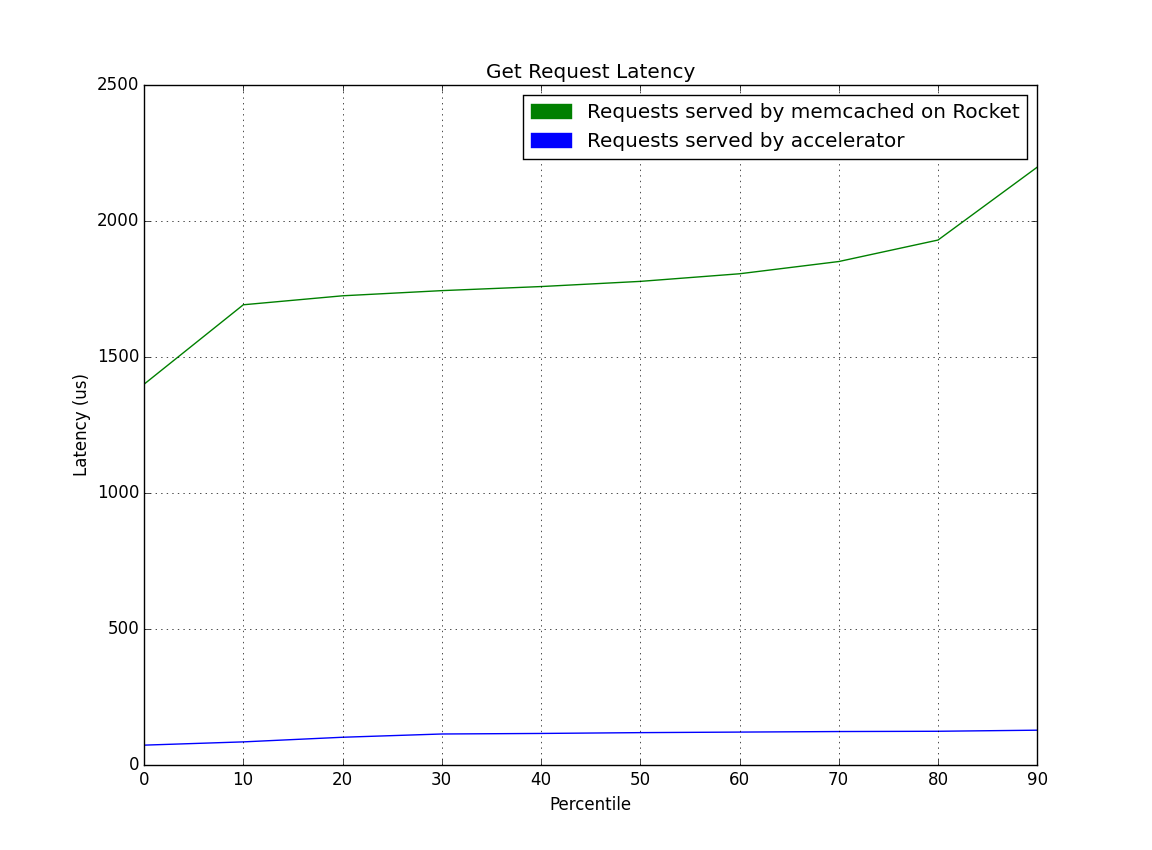
\includegraphics[width=\linewidth]{graph.png}
\caption{Latency of GET requests when only getting 1 key.}
\end{center}
\end{figure}

\begin{figure}[t]
\begin{center}
\label{fig:unif}
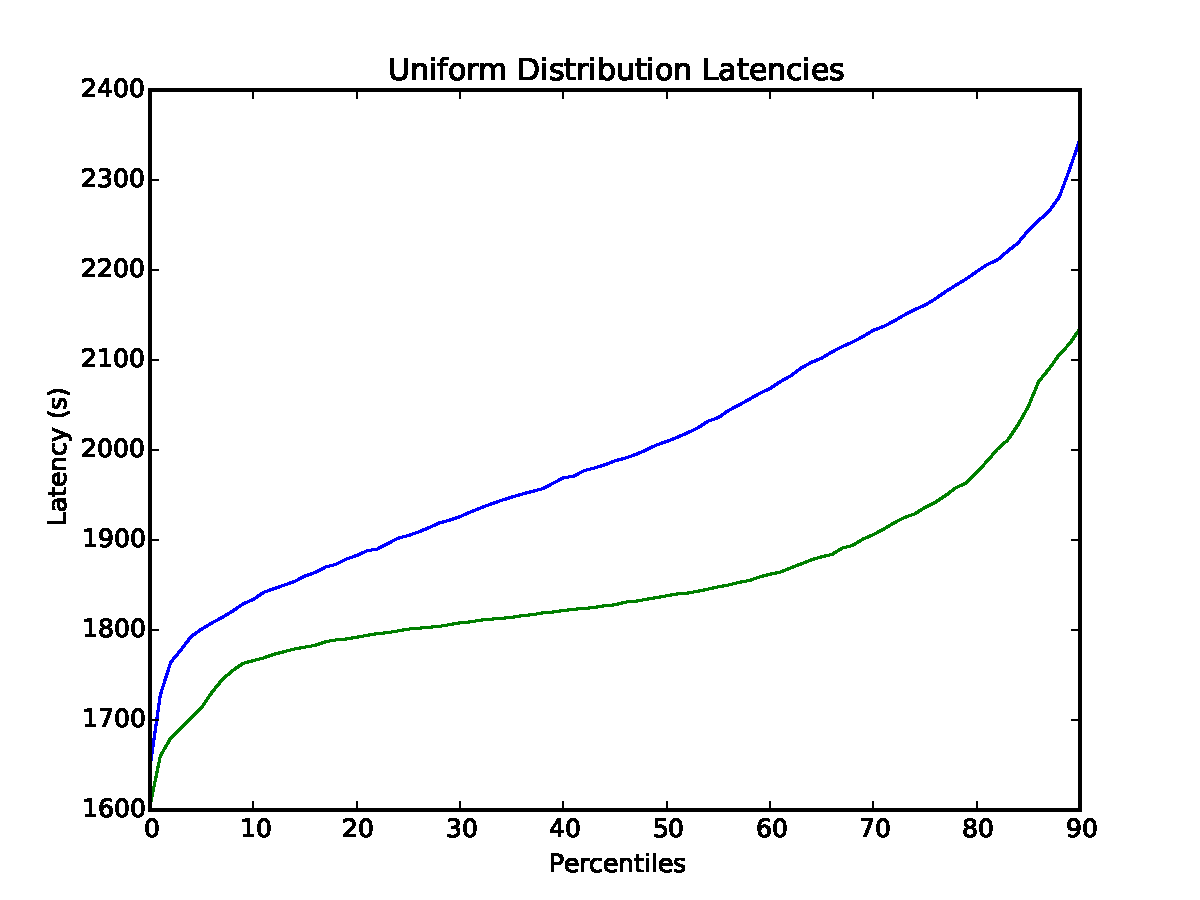
\includegraphics[width=\linewidth]{unif.pdf}
\caption{Latency of GET requests when keys follow a uniform distribution.}
\end{center}
\end{figure}

\begin{figure}[t]
\begin{center}
\label{fig:norm}
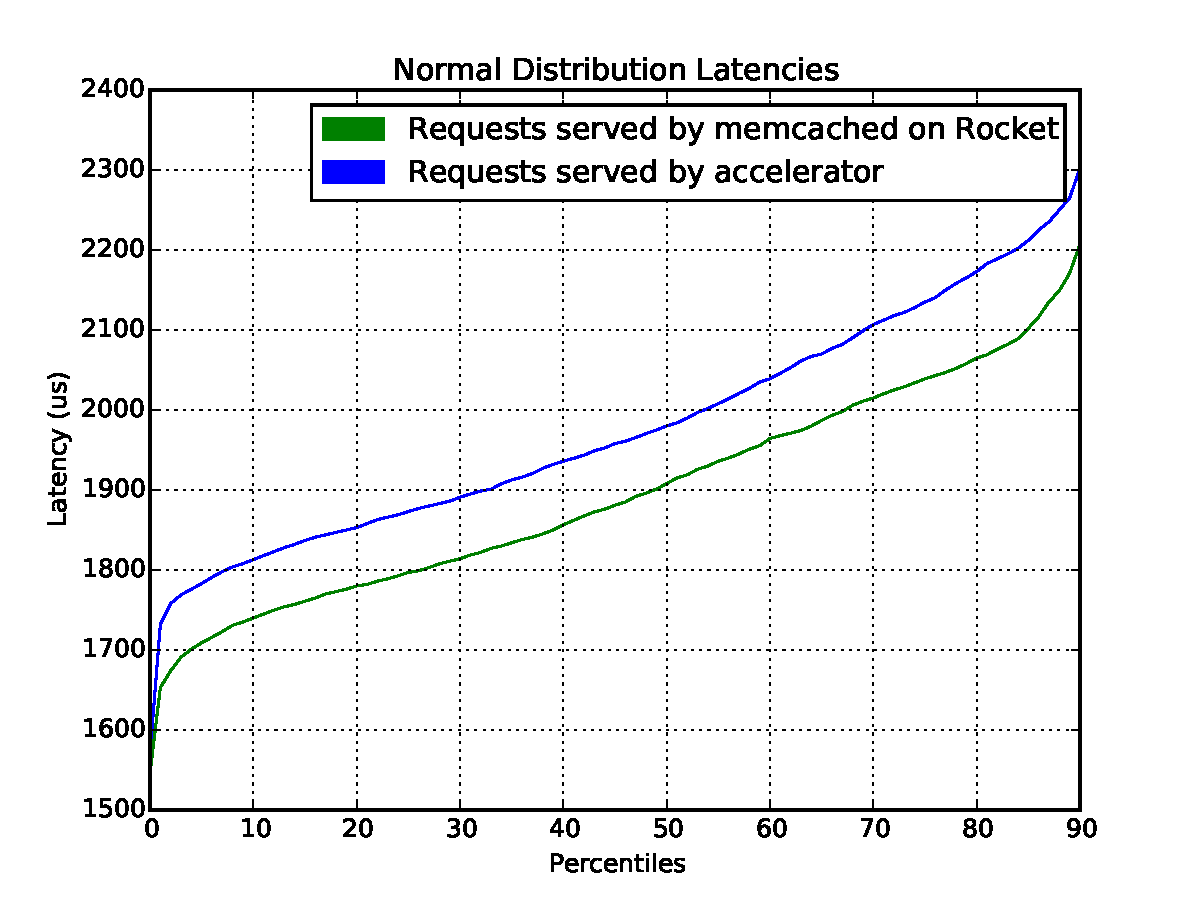
\includegraphics[width=\linewidth]{norm.pdf}
\caption{Latency of GET requests when keys follow a normal distribution.}
\end{center}
\end{figure}

As we see from Figure \ref{fig:one-req}, there is approximatley an order of magnitude
improvement when a key is returned from the accelerator and when a GET request
bypasses the software stack. This shows that for keys on the accelerator, we
should see a very large improvement compared to getting the key from software.

Furthermore, in order to exercise our accelerator fully, we used a bunch of
synthetically generated distributions for the keys. In Figure \ref{fig:unif},
we ran it on a uniform distribution of keys. We see that in this distribution,
the software driven accelerator does only about $40$ to $50$ percent better
than the pure software implementation. The main reason that the average latency
isn't as great is that we are only accelerating a small fraction of the keys.
This necessarily means that a fixed percentage of keys are getting accelerated
at a time, which means that only a small fraction of keys are getting a
speedup. We also note that this happens for other symmetric distributions, like
in Figure \ref{fig:norm} where we used a normal distribution.

\begin{figure}[t]
\begin{center}
\label{fig:pareto}
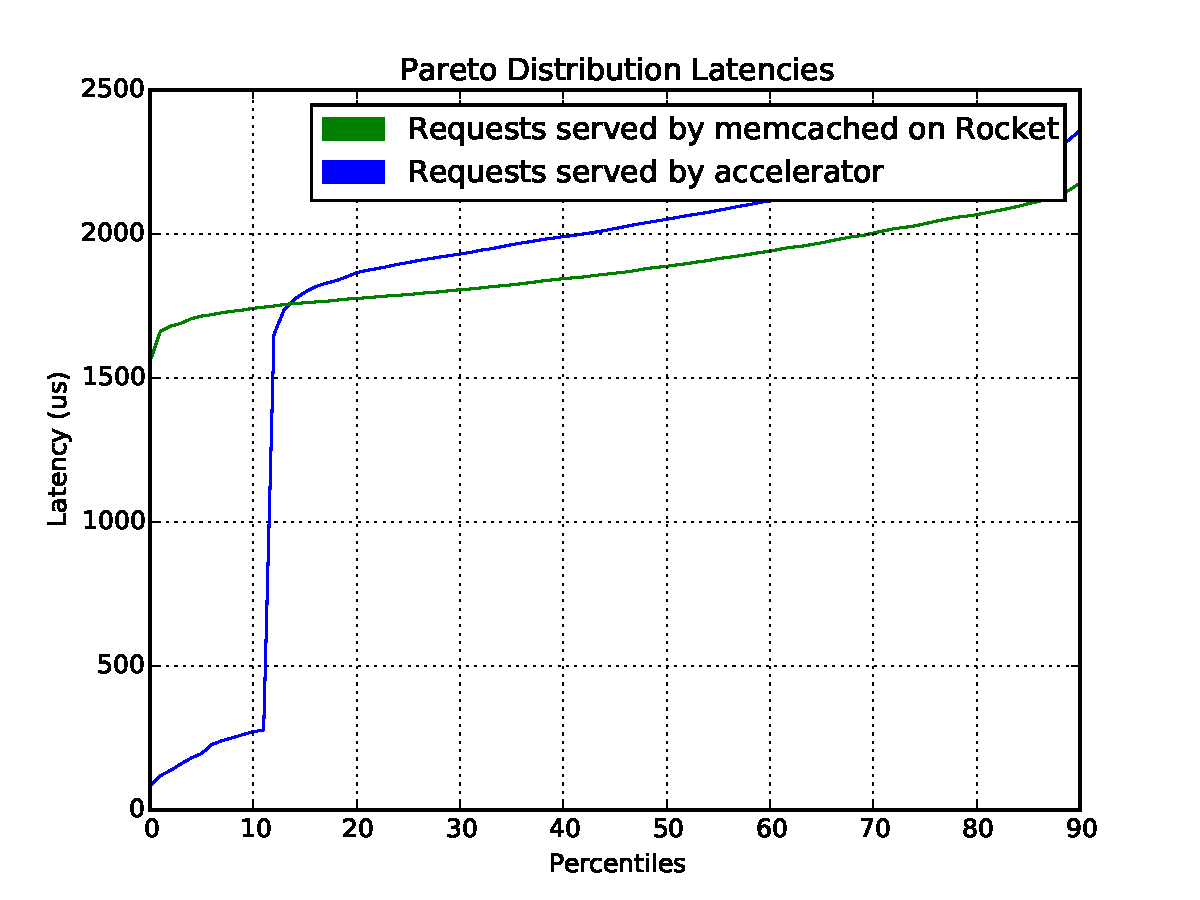
\includegraphics[width=\linewidth]{pareto.pdf}
\caption{Latency of GET requests when keys follow a pareto distribution.}
\end{center}
\end{figure}

\begin{figure}[t]
\begin{center}
\label{fig:etc}
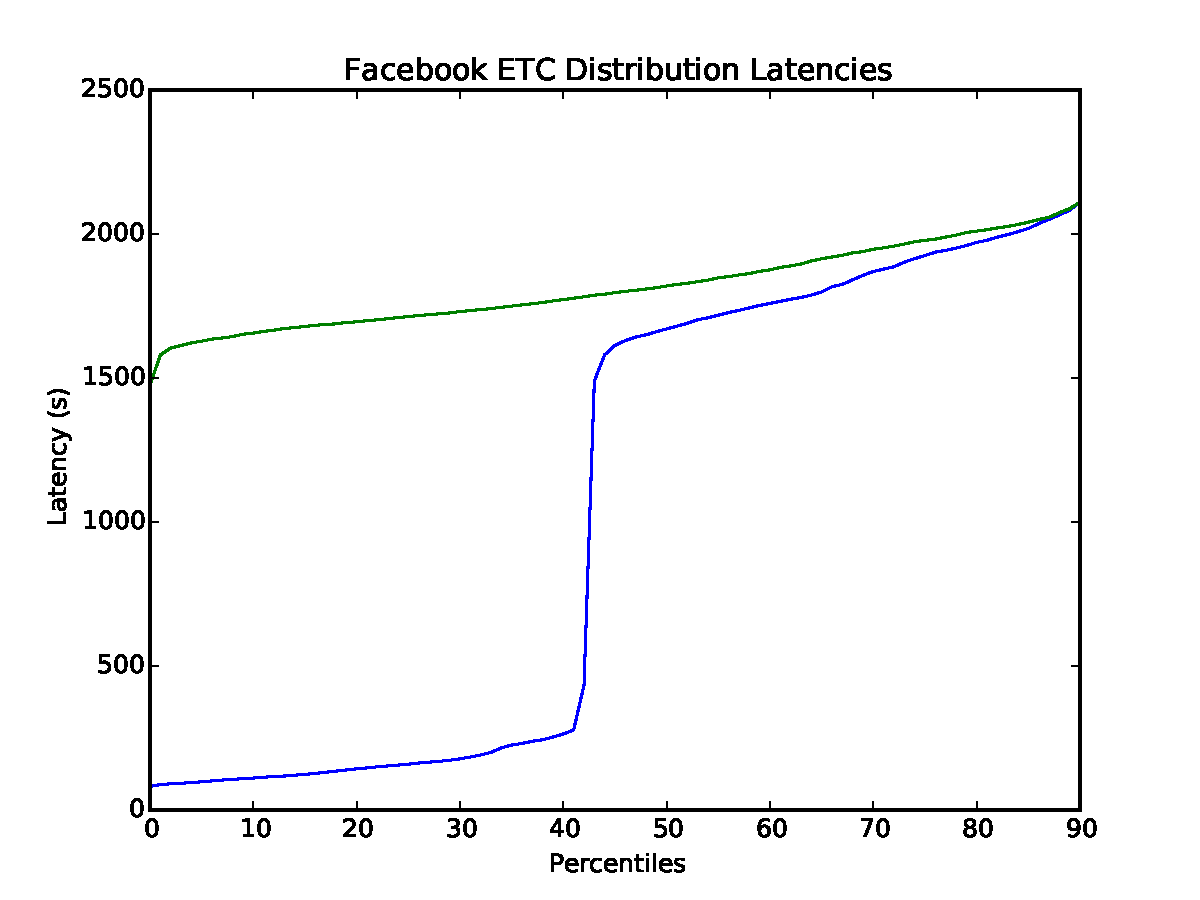
\includegraphics[width=\linewidth]{etc.pdf}
\caption{Latency of GET requests when keys follow the Facebook ETC distribution.}
\end{center}
\end{figure}

For skewed distributions, we see that the benefits of accelerating a small
fraction of the keys is quite large. On our synthetically generated pareto
distribution in Figure \ref{fig:pareto}, we see that the highly skewed keys get the
benefit of a $10$ times improvement over the software implementation. This is
due to the fact that once a hot key gets on the accelerator, it is very hard
for it to get kicked out unless it becomes cold. This is because if it was to
be kicked out by another key, then that key must have been hotter. However, for
highly skewed distributions, the probabilty of two hot keys having a cache
collision is very small. In addition, we see that the software managed
accelerator actually increases the latency for a bunch of keys as well. This is
due to the fact that there is a filter as well, so we are incurring a small
overhead for a large portion of the keys.

Finally, we used the Facebook ETC distribution~\cite{AXFJP2012} in order to see
how our system would fare against a real life workload. In Figure
\ref{fig:etc}, we see that this is a very promising start. $40$ percent of all
requests get a $10$ times improvement in latencies. However, our synthetic
workloads suggest that there are some improvements to be made in our caching
policy that will probably enhance the performance of our system as well.
